\section{Introduction}

\subsection{Search Advertising}

\begin{frame}
	\frametitle{Google Ads}
	\begin{center}
		\includegraphics[scale=0.2]{./resources/images/240px-Google_Ads_logo}
    \end{center}
    \begin{quote}<2->
        \textbf{Google Ads} (previously \textbf{Google AdWords} [...]) is an online advertising platform developed by Google, where advertisers pay to display brief advertisements [...] within the Google ad network to web users. Google Ads' system is based [...] on \textcolor{blue}{keywords} determined by advertisers. Google uses [this characteristic] to place advertising copy on pages where they think it might be relevant.\\
        \flushright \textnormal{(Wikipedia contributors "Google Ads")}
    \end{quote}
\end{frame}

\begin{frame}
    \frametitle{Search Advertising}
    \centering
    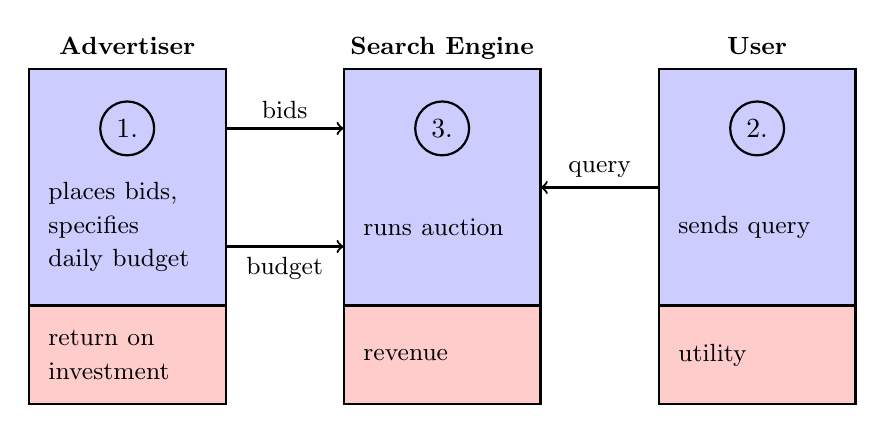
\begin{tikzpicture}
        \begin{scope}[every node/.style={text depth=depth("g")}]
            \path (-5.25,5) -- node[black,above] {\small{\textbf{Advertiser}}} (-2.75,5);
            \path (-1.25,5) -- node[black,above] {\small{\textbf{Search Engine}}} (1.25,5);
            \path (2.75,5) -- node[black,above] {\small{\textbf{User}}} (5.25,5);
        \end{scope}

        \visible<2->{
            \fill[blue!20] (-5.25,2) rectangle (-2.75,5);
            \fill[blue!20] (-1.25,2) rectangle (1.25,5);
            \fill[blue!20] (2.75,2) rectangle (5.25,5);
        }

        \visible<2->{\path (-5.25,2) rectangle node[text width=2cm] {\small{places bids, specifies \mbox{daily budget}}} (-2.75,4);}
        \visible<4->{\path (-1.25,2) rectangle node[text width=2cm] {\small{runs auction}} (1.25,4);}
        \visible<3->{\path (2.75,2) rectangle node[text width=2cm] {\small{sends query}} (5.25,4);}

        \visible<5->{
            \fill[fill=red!20] (-5.25,0.75) rectangle node[text width=2cm] {\small{return on investment}} (-2.75,2);
            \fill[fill=red!20] (-1.25,0.75) rectangle node[text width=2cm] {\small{revenue}} (1.25,2);
            \fill[fill=red!20] (2.75,0.75) rectangle node[text width=2cm] {\small{utility}} (5.25,2);
        }

        \visible<2->{\node[draw,thick,circle] at (-4,4.25) {1.};}
        \visible<3->{\node[draw,thick,circle] at (4,4.25) {2.};}
        \visible<4->{\node[draw,thick,circle] at (0,4.25) {3.};}

        \visible<2->{
            \draw[thick] (-5.25,2) rectangle (-2.75,5);
            \draw[thick] (-1.25,2) rectangle (1.25,5);
            \draw[thick] (2.75,2) rectangle (5.25,5);
        }

        \visible<5->{
            \draw[thick] (-5.25,0.75) rectangle (-2.75,2);
            \draw[thick] (-1.25,0.75) rectangle (1.25,2);
            \draw[thick] (2.75,0.75) rectangle (5.25,2);
        }

        \visible<2->{
            \draw[->,thick] (-2.75,4.25) -- node[above] {\small{bids}} (-1.25,4.25);
            \draw[->,thick] (-2.75,2.75) -- node[below] {\small{budget}} (-1.25,2.75);
        }
        \visible<3->{\draw[->,thick] (2.75,3.5) -- node[above] {\small{query}} (1.25,3.5);}
    \end{tikzpicture}
    \flushleft
    \visible<2->{
        \tikz \filldraw[thick,fill=blue!20] (0,0) rectangle (0.25,0.25);
        \small{Activity}
    }\\
    \visible<5->{
        \tikz \filldraw[thick,fill=red!20] (0,0) rectangle (0.25,0.25);
        \small{Objective function}
    }
\end{frame}

\subsection{Classification}

\begin{frame}
    \frametitle{Matching}
    \begin{definition}
        Let $G = (V,E)$ be a graph. Then $M \subseteq E$ is called \alert{matching} if every vertex $v \in V$ is incident to at most one edge $e \in M$.\\
        \smallskip
        Let $M$ be a matching in $G$. Then:
        \begin{itemize}
            \item<1-> $M$ is called \alert{bipartite} matching if $G$ is bipartite.
            \item<1-> $M$ is called \alert{maximum} matching if $|M| \geq |M^\prime|$ for all matchings $M^\prime \subseteq E$.
        \end{itemize}
    \end{definition}
\end{frame}

\begin{frame}
    \frametitle{Online vs. Offline Algorithm}
    \begin{definition}
        \begin{enumerate}
            \item<1-> An \alert{online algorithm} \textcolor{orange}{ALG} is presented with a \textcolor{blue}{request sequence} $\sigma = \sigma_1, \dots, \sigma_m$. The requests $\sigma_t, 1 \leq t \leq m$, must be served in their order of occurence. More specifically, when serving request $\sigma_t$, \textcolor{orange}{ALG} does not know any request $\sigma_{t^\prime}$ with $t^\prime > t$.\\
            \smallskip
            Serving requests affects the \textcolor{blue}{objective function} value attained by \textcolor{orange}{ALG}, and the goal is to \textcolor{blue}{optimize} the value of the objective function attained on the entire request sequence.
            \item<2-> An \alert{offline algorithm}, on the other hand, is an omniscient algorithm that knows the entire request sequence in advance and can compute an optimum output.
        \end{enumerate}
    \end{definition}
\end{frame}

\begin{frame}
    \frametitle{Online Bipartite Matching Problem}
    \begin{block}{Online Bipartite Matching Problem}
        \textbf{Given:} A bipartite graph $G = (U,V,E)$, where:
        \begin{itemize}
            \item<1-> $U$ arrives offline
            \item<1-> $V$ arrives online
            \item<1-> When a vertex in $V$ arrives, its neighbors in $U$ are revealed
        \end{itemize}
        \smallskip
        \visible<2->{
            \textbf{Task:}
            \begin{itemize}
                \item<1-> An arriving vertex needs to be matched to an available neighbor (if any)
                \item<1-> A match once made cannot be revoked
            \end{itemize}
            \smallskip
        }
        \visible<3->{\textbf{Goal:} Maximize the size of the matching}
    \end{block}
\end{frame}

\begin{frame}
	\frametitle{Adwords Problem}
	\begin{block}{Adwords Problem}
		\textbf{Given:} A bipartite graph $G = (U,V,E)$, where:
		\begin{itemize}
			\item<1-> Each vertex $u \in U$ has a budget $b_u$
			\item<1-> Each edge $(u,v) \in E$ has a bid $c_{u,v}$
		\end{itemize}
		\smallskip
		\visible<2->{
            \textbf{Task:}
            \begin{itemize}
                \item<1-> When an arriving vertex $v \in V$ is matched to a neighbor $u \in U$, then $u$ depletes $c_{u,v}$ amount of its budget
                \item<1-> When a vertex depletes its entire budget, then it becomes unavailable
            \end{itemize}
            \smallskip
        }
		\visible<3->{\textbf{Goal:} Maximize the total money spent}
	\end{block}
\end{frame}

\begin{frame}
    \frametitle{Landscape of Problems}
    \centering
    \begin{tikzpicture}
		\draw[very thick,orange] \orangeellipse;
		\draw[very thick,violet] \violetellipse;
		\draw[very thick,red] \redellipse;
	\end{tikzpicture}
\end{frame}